% LaTeX template for ECE 496 Reports
% Last updated 27 January 2014 by Ben Ujcich

% Copyright (C) 2014 Laura Clancy, Julian Coy Katelyn Fry,
%                    Gregory Stephens, and Ben Ujcich

%% CHANGE REPORT TITLE HERE
\newcommand{\reporttitle}{
2-Wheeled Segway Robot Design:
Final Report
}

%% HEADER/PREAMBLE INFORMATION

\documentclass[11pt]{report}
\usepackage[T1]{fontenc}
\usepackage[utf8]{inputenc}

% "The font should be 11pt Times New Roman"
\usepackage{mathptmx}               

% "The body of the paper should use 1" margins on all sides."
\usepackage[margin=1in]{geometry}

% "Pages must be numbered, starting with 1 on the first page in the body of the report.
% The cover page should not be numbered. 
% Page numbers should be in the bottom-right corner of the page."
\usepackage{fancyhdr}
\pagestyle{fancy}
\fancyhead{}
\fancyfoot{}
\renewcommand{\headrulewidth}{0pt}
\fancyfoot[R]{\thepage}

% Set up customized spacing
\usepackage{setspace}

% Allows for Trademark Symbols
\usepackage{textcomp}

% Remove spacing between items in lists
\usepackage{enumitem}

% Remove extra spacing between titles of sections and subsections
\usepackage{titlesec}
\titlespacing\section{0pt}{0pt plus 4pt minus 2pt}{0pt plus 2pt minus 2pt}
\titlespacing\subsection{0pt}{0pt plus 4pt minus 2pt}{0pt plus 2pt minus 2pt}
\titlespacing\subsubsection{0pt}{0pt plus 4pt minus 2pt}{0pt plus 2pt minus 2pt}
\titlespacing\paragraph{20pt}{0pt}{10pt}

% Set up BibTeX integration using IEEE citation format
\usepackage{cite}
\bibliographystyle{ieeetr}
\usepackage{url}

% Set bibliography to have a section header rather than chapter header
\makeatletter
\renewenvironment{thebibliography}[1]
     {\section*{Works Cited}% <-- this line was changed from \chapter* to \section*
      \@mkboth{\MakeUppercase\bibname}{\MakeUppercase\bibname}%
      \list{\@biblabel{\@arabic\c@enumiv}}%
           {\settowidth\labelwidth{\@biblabel{#1}}%
            \leftmargin\labelwidth
            \advance\leftmargin\labelsep
            \@openbib@code
            \usecounter{enumiv}%
            \let\p@enumiv\@empty
            \renewcommand\theenumiv{\@arabic\c@enumiv}}%
      \sloppy
      \clubpenalty4000
      \@clubpenalty \clubpenalty
      \widowpenalty4000%
      \sfcode`\.\@m}
     {\def\@noitemerr
       {\@latex@warning{Empty `thebibliography' environment}}%
      \endlist}
\makeatother

% Set up math
\usepackage{amsmath}
\usepackage{amsfonts}
\usepackage{amssymb}

% Set up graphics
\usepackage{graphicx}
\usepackage{float}

% Set up tables
\usepackage{tabularx}
\usepackage{booktabs}

%% START OF DOCUMENT

\begin{document}

% "The main body of text should use 1.5 spacing"
\begin{spacing}{1.5}

% Suppress page numbering on first page
\thispagestyle{empty}

% Title
% "The title should be centered and written in approximately 22pt font."
\vspace*{72pt}
{
\huge
\begin{center}
    \reporttitle
\end{center}
}
\vspace{72pt}

% Team Number
% "The Team number should be centered and written several lines below the title and should use a
% similar size font as the title."
{
\huge
\begin{center}
  Team SR03
\end{center}
}

% Team Members
% "Directly below the team identifier, team members should be listed alphabetically by last name, one
% per line, in approximately 14pt font. The column of names should be approximately centered on
% the page, but the names within the column should be left justified (so they all start at the same
% horizontal position)."
{
\Large 
\begin{center}
  \begin{tabular}{l}
    Laura Clancy \\
    Julian Coy \\
    Katelyn Fry \\
    Gregory Stephens \\
    Ben Ujcich
  \end{tabular}
\end{center}
}

% New page and reset page numbering
\clearpage
\setcounter{page}{1}

%% START EDITS BELOW %%




\section*{Problem Statement} %(0.5 pages)

The desired goal of the senior design project was to build a functioning robot that could successfully balance and move on two wheels as directed by the user. This design was meant to be based on the commercial Segway robot but created on a much smaller scale. The design requirements of the project included: 1) the robot will be roughly 18 inches high and no more than 9 inches wide and 2) without the use of RC Servo motors, the miniature Segway robot must be able to move forwards, backwards, and turn left and right. In our particular implementation, an individual power amplifier was constructed and the entire device was run from a single DC voltage supplied to the system. The system was controlled with the Tiva C Series TM4C123G LaunchPad and a Raspberry Pi computer. Our team encountered many difficulties in accomplishing the goal of balancing as outlined throughout this report.

\section*{Specifications}
We were given the following specifications to meet minimum requirements for the project \cite{Requirements}:
\begin{itemize}[noitemsep,nolistsep]
    \item The robot should stand roughly 18 inches high.
    \item The real time component of the system must be implemented using the Tiva C Series TM4C123G LaunchPad.
    \item The power for the motors must be provided using your own selected electronics.
    \item The only power supplied to the system should come from a single DC voltage 
source.
    \item A remote control must be implemented for the robot.
    \item The robot should be robust to significant perturbations.
    \item The primary performance metric will be the ability of the robot to traverse reasonable flat ground robustly. 
\end{itemize}

We based our design off of the following design principles:
\begin{itemize}[noitemsep,nolistsep]
    \item \emph{Choose off-the-shelf parts} rather than self-made parts whenever possible.
    \item \emph{Reuse and expand on open-source software libraries} to avoid spending time writing code that duplicates functionality that already exists elsewhere (and is likely more robust).
    \item \emph{Keep the hardware simple} by using the least amount of hardware necessary for operation to avoid additional potential points of failure.
    \item \emph{Modularize systems and components}. Each component should do one thing and do it well.
\end{itemize}

\section*{Final Design}

    \subsection*{Subsystem Description}
    
    Figure \ref{SubsystemInteraction} shows the subsystem interactions between the Tiva board, the battery, optical sensors, DC motors, the driver chip, the controller, the Raspberry Pi, and the gyroscope/accelerometer.
    
    \begin{figure}[H]
                \centering
                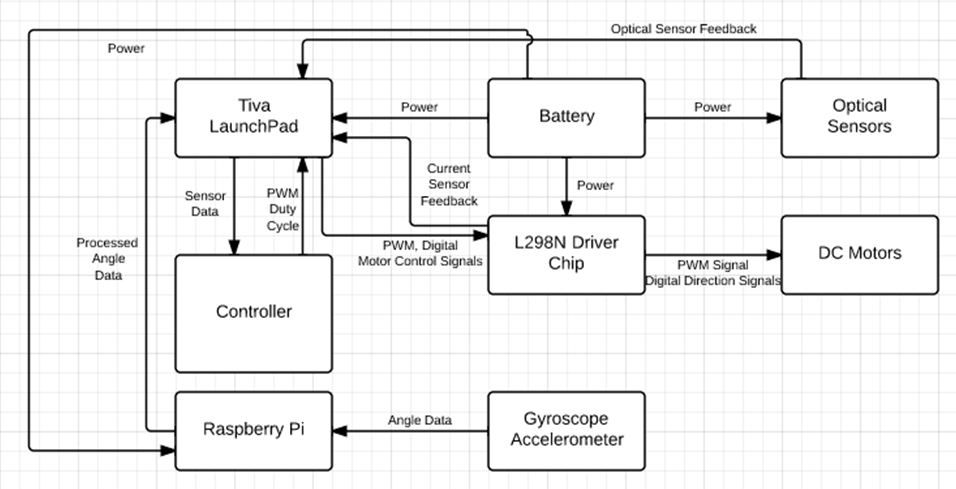
\includegraphics[width=0.5\textwidth]{SubsystemInteraction}
                \caption{Subsystem Interactions Diagram}
                \label{SubsystemInteraction}
            \end{figure}

        \paragraph{Power Electronics}
        
        The power electronics design was developed to satisfy the needs of the purchased 29:1 DC Gearmotors. A dual-channel H-Bridge was used to control both motor direction and speed. The L298N driver chip requires six total signals from the Tiva LaunchPad to properly control both motors. Two digital outputs are used to control the direction a motor. Signals of 0-1 tell the motor to turn forwards, signals of 1-0 tell the motor to turn backwards, and if the two signals are the same the motor stops turning. The driver chip also uses a PWM signal from the Tiva chip for each motor to control speed. Because the Tiva outputs a 3.3 V signal, a 2N3904 transistor pull-up circuit was built with two 10k$\Omega$ resistors to pull up the logic voltage to 5 V (the driver chip expected a 5 V input). A higher PWM duty cycle means that a higher average voltage is delivered to the motors which increases their speed. Eight protection Schottky diodes and two 100 nF capacitors were added to the driver chip circuit as seen in Figure \ref{PowerElectronics} in order to protect the motor terminals from voltage spikes due to incorrect wiring and smooth out the power signals, respectively. 
        
            \begin{figure}[H]
                \centering
                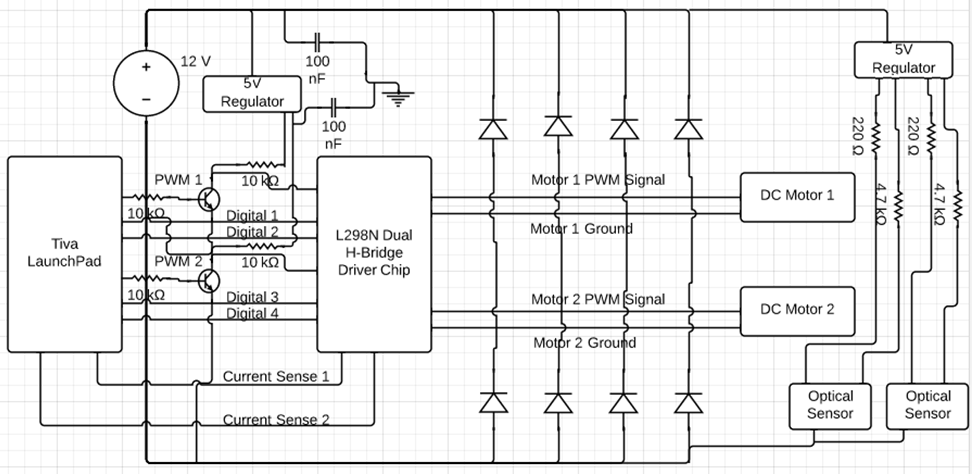
\includegraphics[width=0.5\textwidth]{PowerElectronics}
                \caption{Power Electronics Subsystem Circuit Diagram}
                \label{PowerElectronics}
            \end{figure}
        
        \paragraph{Sensors}
        
        Two current sensors were utilized onboard the miniature Segway robot. They were located internally in the L298N driver chip. The L298N monitored the current in both motor circuits and sent a corresponding analog voltage between 0 and 2 V. This current feedback was essential to the controller design and required gains to be tuned with the current sensor feedback. Optical sensors were used in place of encoders to report the real-time speed of the motors to the controller. The QRD1114 optical sensors were mounted to the bottom of the lower mount facing out towards the inside of the wheels. Black and white print out circles were made and attached to the inside of the wheels. The circles had triangular segments, alternating white and black every ten degrees. The optical sensors use infrared beams to detect white/black transitions. In a 0 to 5 V range, it will return a low or high voltage depending on if the sensor sees white or black. By counting the transitions and interpreting over time, a motor speed could be calculated.
        
        Embedded in a BOOSTXL-SENHUB board, an MPU-9150 9-axis sensor chip was used for position and acceleration measurements.  The MPU-9150 is a composite sensor that has a gyroscope, accelerometer, and magnetometer.  The sensor is capable of combining all three component sensor readings into one using InvenSense's MotionFusion{\texttrademark} firmware.  This system allows recalibration of the sensors to be performed at run-time which eliminates the need for zero-drift calculations.  The "sensor fusion" algorithms allowed us to focus on integration of the data from the sensor instead of worrying about how to ensure data integrity.

        \paragraph{Battery Power System}
        
        A 12V NiMH battery package was decided on as the optimal power supply for our robotic system. The package that was decided upon was a custom fabricated 3800mAh 12V supply from Batteryspace.com – a company that specializes in modularpower solutions for hobbyist projects. The 12V pack consists of 10 individual 1.2V NiMH cells strung together in series and secured together using the manufacturers wrapping. We chose to use 6 inch 18AWG bare wire leads for our connection purposes. The purpose of the battery power supply was to remove the need for all external connections/wires/tethers from the robot, and it succeeded in supplying more than enough power for the robot to be operational.
        
        \paragraph{Controller}
        
        The purpose of the balancing system is to ensure that the robotic system will maintain a desired position determined by the microcontroller subsystem. The controller used three control loops: one for angular position, velocity, and current. 
        
        The first control loop was set to control angular position.  The desired position, called the desired $\theta_2$ value as shown in \cite{Groff}, is used as an input to the balancing system by the microcontroller subsystem. The actual angle position of the robotic system is derived by measurements from a gyroscope (which is part of the sensing subsystem). The gyroscope measures angular velocity and as such, this value is integrated twice to provide the actual angle position $\theta_2$. To balance the system at rest, the desired $\theta_2$ was set to zero. To move the robot either forwards or backwards, the desired $\theta_2$ was set to a positive or negative angle respectively. 
        
        The second loop was set to control velocity.  The desired velocity, called the desired $\Omega_1$ value as shown in \cite{Groff}, was set to 0 for balancing and to a small value for movement.  The actual $\Omega_1$ was measured from a set of optical sensors.  These sensors measured the number of color changes from black and white pinwheels mounted on the wheels of the robot.  The number of changes in a certain amount of time was used to determine the speed of the robot.  
        
        These first two loops each produced a torque signal.  These two signals were added to create an overall torque signal.  This value was first divided by 2 in order to account for the fact there are two motors.  The overall torque signal is the torque needed for the entire system.  Since there are two motors, this value must be divided between the two.  This value was then divided by $k = .1335$ to create a current signal.  This constant $k$ was determined by dividing the stall torque and current of our motors.
        
        The transformed signal was then treated as the desired current, or desired $i$.  This value was then compared to values obtained from current sensors built into the motor driver chip.  These two values were used to create an error signal that was minimized using a gain.  This signal acted as a modifier for the desired $i$ and as such was added to a feed forward loop for the desired $i$.  This signal was then transformed into a duty cycle.  The current was multiplied by the armature resistance $R_A$ of the motors to calculate the armature voltage $V_A$.  Then $V_A$ was divided by the source voltage $V_S$ to calculate the duty cycle, $k$.  Finally, the duty cycle was then used to generate a PWM to be sent to each motor.  This transformation and values of the variables are shown below in Equation \ref{PIDControlEquation}.
        \begin{align}
    k &= \dfrac{i \cdot  R_A}{V_S} = \dfrac{i \cdot 122 \Omega}{6 V} \label{PIDControlEquation}
\end{align}

The complete controller is shown below in Figure \ref{ControllerDiagram}.

\begin{figure}[H]
                \centering
                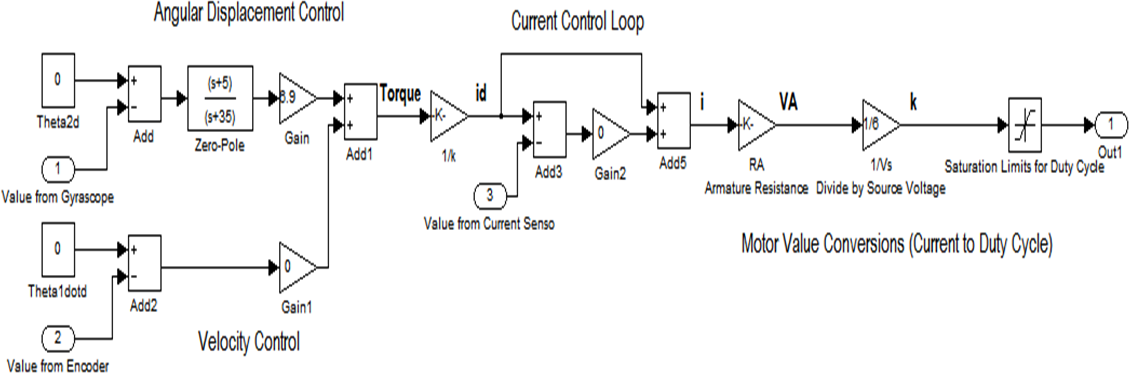
\includegraphics[width=\textwidth]{ControllerDiagram}
                \caption{Controller Diagram}
                \label{ControllerDiagram}
            \end{figure}
        
        \paragraph{Microcontrollers}
        
        There are two microcontrollers used in the final design.  A Tiva C Launchpad, or EK-TM4C123GXL, and a Raspberry Pi.  Each microcontroller ran specific software functions for the entire robot.  The Tiva C was flashed with motor controlling software, while the Raspberry Pi housed motion sensing software.

        The Tiva C operates an ARM Cortex-M4F processor with USB 2.0 device interfacing, a hibernation module, and a motion control pulse-width modulator (MC PWM) module.  The Tiva C also features multiple connection pins to facilitate hardware expansion and external interfacing.  In the final design, the Tiva C was connected to the Raspberry Pi, the motor drivers, and optical sensors.  This made the Tiva C micro the central data processing hub for the entire system.  The multiple PWM generation capability was the key reason to utilizing the Tiva C as the motor controller logic operator.  Without multiple PWM signals, it would be incredibly difficult, if not impossible, to generate two separate motor signals.

        The Raspberry Pi was chosen as a secondary microcontroller to interface with the MPU-9150 motion sensor housed in the BOOSTXL-SENSHUB board.  The Raspberry Pi was connected to the Tiva C via an 8 bit parallel GPIO connection.  This connection was utilized to stream location and motion data from the MPU-9150 to the Tiva C for controller calculations.

        \paragraph{Mechanical System}
        
        The motors used for the final design were Pololu 29:1 DC Gearmotors.  They were powered through the L298N dual H-Bridge motor driver and mounted directly below the lower wooden mounting block using aluminum L-brackets. Aluminum mounting hubs were used to attach the motor shafts to a pair of Pololu 90mm by 10 mm wheels. 
        
        The physical build that was decided upon consisted of two pine wood platforms – one a 6 inch square and the other a 4 inch square, both $\frac{1}{2}$ inch thick, connected by an 18 inch stainless steel threaded rod sheathed by a hollow aluminum tube. The 6 inch square was fastened to the top of the steel rod, while the 4 inch square served as the base of the robot. The motors/wheels were attached to the underside of the base plate. The idea was to put the processor and the battery at the top to help raise the robot’s center of gravity, creating an easier dynamic system for the controller to balance. However, after realizing we needed two processors instead of one, it was decided to move the battery to the base to allow the processors to sit together on top. 
        
        \paragraph{Communications}
        
        The communications subsystem that was to be implemented on the robot was the Emmoco EDB-BLE development board using Bluetooth 4.0 Low Energy (BLE) standard. The reason for using the board was that by having a separate development board for Bluetooth communications, we would be able to debug the wireless protocols seperately from the rest of the system in order to save on development time and costs. Additionally, the EDB-BLE development board provided the em-framework to allow for building control apps for moobile devices such as Android and iOS phones.
        

    \subsection*{Subsystem Discussion}
    
        \paragraph{Power Electronics}
        
        The power electronics design was chosen because it was the only stable way to properly supply both motors with the needed current. The dual channel H-Bridge is the best and cheapest solution to implement both directional and speed motor control. Each channel can supply up to 2 A continuously. In the original design, just a power amplifier was suggested to power both motors. This would not have worked successfully and the idea stemmed from a lack of knowledge concerning H-Bridges. After doing more research and exploring the capabilities of H-Bridges it was discovered that it would be the only stable and viable option for the given design requirements.
        
        \paragraph{Sensors}
        
        Originally, neither of these sensors were part of the overall design. After developing the control scheme, it was discovered that both the motor positions and currents needed to be monitored and used as feedback. The L298N dual H-Bridge driver chip had built-in current sensors that fed back to the Tiva and the control scheme. The optical sensors were used as a work-around because the motors were not purchased with encoders. Instead of purchasing new motors, the optical sensors were used as a replacement to still send feedback on motor position to the controller.
        
        The concept of a self-calibration motion sensor was wonderful.  We opted for the MPU-9150 solely based off of its highly rated accuracy and reliability.  Unfortunately, we did not anticipate the difficult of communication between the MPU-9150 and the Tiva C via Simulink.  The code that was provided was specifically for the MPU-6150's dataset and would not interface with the MPU-9150 at all.  The inability to communicate with our sensor was probably the largest drawback in the entire project.  The entire premise of obtaining a secondary microcontroller was essentially created by the need to interface with our sensor.  Fortunately, once an interface was created the MPU-9150 provided reliable and accurate sensor data for the segway.

        \paragraph{Battery Power System}
        
        The primary concerns for the battery supply were total discharge capacity and safety. After researching multiple types of battery packs, NiMH cells were deemed to be the safest option, as they posed the least likelihood to explode (advice from a seasoned robotics engineer), and they don’t have the capacity to leak toxic chemicals like many other types of battery packs. As for discharge capacity, during motor testing, the maximum observed current draw from both of the motors was around .7 Amps each. It was decided that having a battery capable of powering more than double that load for at least half an hour would be sufficient for all of our testing and demonstration purposes. As such, a 3800mAh pack fit our bill, because it would be able to power two times our anticipated motor load (2.8 Amps) for more than an hour without the need to recharge. This subsystem in our robot matches the expectations set forth in the preliminary report.
        
        \paragraph{Controller}
        
        The control loop for the angular position employed a lead compensator to provide a steady system and to minimize the distance between the desired $\theta_2$ and the actual $\theta_2$ (i.e. minimizing the error).  This was necessary because without the addition of a new pole, the root locus plot for this variable would have a pole that never entered the left hand side of the plane and thus would never be stable.  A further discussion of this is shown in Appendix B.  The control loop for the velocity and the control loop for the current only needed to use a simple gain rather than employ a compensator or controller.  Unlike the root locus plot for the angular position, the zeros and poles for these plots moved to the real half of the plane without having to introduce a new pole.  
        
        
        \paragraph{Microcontrollers}
        
        The Tiva C was a design requirement for real time control of the robotic system.  To this effect, the Tiva C was utilized well.  The major drawback that was experienced with the Tiva C came from its communication abilities.  Although the Tiva C is more than capable of performing I$^2$C and SPI communication, there were no support packages available to allow this functionality to be integrated into our robot.  This difficulty in communication was what spawned the idea of using a secondary microcontroller to communicate with the MPU-9150.  The microcontroller selected for this task was a Raspberry Pi.

        To reiterate, the Raspberry Pi was chosen to remove limitations with I$^2$C protocol communication between the MPU-9150 and the Tiva C.  Although the Tiva C and BOOSTXL-SENSHUB boards were designed to interface, there is unfortunately no Simulink support package written for this type of interfacing.  Due to the complexity of writing a new I$^2$C device library for Simulink, the Raspberry Pi was selected as a viable alternative to writing an I$^2$C Simulink library.

        Once the sensor data extraction code was written for the Raspberry Pi, an 8 bit data stream was sent via parallel communication to the Tiva C.  This allowed us to achieve a much higher data rate for our sensor that was once thought possible.  There were two major drawbacks to using the Raspberry Pi as go-between for the sensor and the Tiva C.  The first was power consumption.  Although the Raspberry Pi and Tiva C are both very low consumption devices, running both at the same time was a significant waste of energy.  The second drawback was simply communication integrity.  The more wires that data crosses, the more likely it is to become corrupted.  Fortunately, we were able to curb the second issue by using direct communication via 8 GPIO lines.  Any significant change in data readings, due to transmission issues, was easily traced using numerical feedback from the Raspberry Pi operating system.

        \paragraph{Mechanical System}
        
        The original motor design did not change in the final design. DC motors were used as originally proposed and mounted in a stable and efficient location.
        
        Our final mechanical build looks quite different from most of the other competitors’ models. Where most designs tried to create a sleek profile and utilize a minimalist approach, our team decided that a durable wood and steel build would provide the best chance of success. We chose to use dissimilar wooden platforms in an attempt to raise the system’s center of gravity. According to dynamics equations given in the course, theoretically, the higher the center of mass, the easier it is to implement a controller for balance. Thus, we attempted to place the heaviest components as far above the base of the model as possible. The durability over acrylic that we gained from using wood and steel was also a factor as we expected to have many crashes during balance testing.
        
        \paragraph{Communications}
        
        The communications system was difficult to interface with due to the use of two frameworks (em-framework and the Tiva framework) integrating with Simulink. Some time was spent attempting to write custom blocks for the Simulink model but ultimately proved to be too time consuming. We determined that our efforts would be better spent on getting the robot to balance rather than getting the communications system working.

\section*{Cost Accounting}

See Appendix A for the full cost accounting tables.

\begin{itemize}[noitemsep,nolistsep]
    \item \textbf{Development costs:} \$369.46 (the total cost of all items used during the semester, purchased and donated)
    \item \textbf{Out of Pocket Development Costs:} \$354.49 (the total cost of all items purchased during the semester)
    \item \textbf{Final Artifact Cost:} \$318.88 (the total cost of all items that appear in the final design, purchased and donated)
    \item \textbf{Out-of-Pocket Final Artifact Cost:} \$308.95 (the total cost of all items purchased and used in the final design)

\end{itemize}

\section*{Performance Characterization and Discussion}

    Comparing the testing plans as set in the preliminary report to what was accomplished, we were not able to carry out most of the tests due to the inability of the Segway robot to balance correctly. Individual component testing plans and results are outlined below:
    
        \paragraph{Balancing System} \emph{"To test the gyroscope, the robot will be moved to different angles while the output of the gyroscope is recorded."} We were able to correctly determine that the Raspberry Pi was reading the gyroscope data correctly and sending it to 8 of the GPIO pins in the Tiva as an unsigned 8-bit integer with precision of one degree.
        
        \paragraph{Controller} \emph{"However, the majority of testing that will take place for this subsystem will come from the process of tuning the gains to write the PID controller.... While the system is running, different scopes will be used to compare the actual position with the desired position.  This data will be continually collected as the gains are adjusted to reduce the error."} We were not able to tune the controller to any signficiant degree due to lack of feedback data from the Tiva. The Simulink software provided with the Tiva was not able to correctly work when attempting to access real-time data to use to plot graphs of the feedback. Had we known the difficulties in integrating the Tiva with Simulink, we would have used the xPC to tune the gains of the controller.
        
        \paragraph{Motors} \emph{"For the preliminary torque test, the motors will be connected to the wheels and sent signals to move at different speeds. The speed of the rotating wheel will be visually observed and the control speeds will be calibrated in order to determine what needs to be sent to the motors to achieve minimum and maximum speeds."} The PWM signal was generated by the Tiva, and we tested that the PWM signal was correctly being sent from the board by using an oscilloscope. We tested the signal with duty cycles between 10 and 90 percent, and the motor's speed was responsive to the output.
        
        \paragraph{Power Amplifier and Voltage Regulator} \emph{"Both the power amplifier electronics and voltage regulator only need to be tested using a multimeter. The input voltages will be tested to verify their compatibility with the circuit components. Each electronic device will then be wired into the system and its voltage and current outputs measured before connecting them to the entire system."} The voltage regulator worked correctly, and we experienced no problems in powering the Tiva board or the Raspberry Pi computer.
        
        \paragraph{Mechanical System} \emph{"The majority of the testing for this system will be to test for robustness and durability.  This testing is necessary to ensure that the more delicate parts of the overall system will be protected.  Experimentation will also be done with the length of the PVC pipe and the mass of the counterweight to determine the best configuration to ensure a safe, durable, and controllable system."} The mechanical system was designed in such a way as to balance the weight of the components symmetrically so as to not have a significantly uneven weight pattern present. Important components such as the Tiva board and the Raspberry Pi were placed on the top of the robot to prevent them from being damaged if the robot were to fall over; similarly, the gyroscopic sensor was placed on the pipe to both ensure that an accurate angle measurement could be determined and that it would not be damaged.
        

\section*{Project Postmortem}

    \subsection*{Technical Postmortem}
    
    The strengths of the final design for this project include robust power electronics, a completely onboard electrical and mechanical system, and the use of a Raspberry Pi microcontroller in conjunction with the Tiva LaunchPad. The power electronics included an L298N dual H-Bridge driver chip that was capable of supplying a total of 4 Amps (2 Amps per motor) continuously. With built-in current sensing, the driver chip functioned properly to both control the motors and provide vital feedback to the controller. Both motor directional and speed controls were tested before the power electronics were mounted on the mechanical system and were found to work perfectly. The PWM duty cycle was directly proportional to the average voltage and therefore speed of the motors. 
    
    All of the electronics used to monitor and control the system were located onboard the mechanical system. No tethers to any equipment on the desktop were necessary due to the use of a battery and several voltage regulator chips. This was an important strength of the system because it allowed for untethered testing and movement of the system. 
    
    The final strength was the utilization of the Raspberry Pi microcontroller in conjunction with the Tiva LaunchPad. The Raspberry Pi processes the gyroscope and accelerometer data much more quickly than the Tiva LaunchPad – then the processed angle value was sent from the Raspberry Pi to the Tiva LaunchPad to feed into the controller. However, the Raspberry Pi also represented a weakness in the final system design. In order to begin proper operation, the Raspberry Pi requires 30 seconds to boot, during which time no sensor data is being read. This design choice was a byproduct of the system’s largest weakness: communication of sensor data with the purchased MPU9150 gyroscope and accelerometer sensor package.Although designed to work with the Tiva LaunchPad, the necessary open source code to interface the two did not exist. By the time this was researched and discovered, very little could be done in terms of code-development due to time limitations. Therefore, the Raspberry Pi was instituted as a work-around. Additionally, setbacks in the implementation of the gyroscope and accelerometer as well as a lack of graphical data and error signals led to having a controller that was not fine-tuned. Although initial values were developed, the lack of graphical signals meant that the controller was never able to be tuned beyond the initial guesses from the root locus plots. 
    
    The project was also hindered for financial reasons. As projects were self-funded, the cost of the project was an important factor. Because of this, motors without encoders were purchased to save money. Later during the development of the control scheme it was discovered that encoders were an integral part of the controls. This led to optical sensors being a less accurate but plausible work-around for the lack of motor encoders. 
    
    The final design would be capable of much more if time restrictions and management issues had not arisen. The entire power electronics system was fully and perfectly functional with the Tiva LaunchPad until mounting everything onto the mechanical system. With more time, graphical sensor data and error signals could have been obtained, and the control gains could have been finalized and the system could have performed at a much higher level than demonstrated.In retrospect, two things stand out as alternatives that would have greatly improved the abilities of the final design. First, starting to analyze and communicate the sensor data from the gyroscope and accelerometer at a much earlier date would have brought issues to light much sooner when they could still be fixed. Secondly, more time could have been spent attempting to make the feedback controls function on the Quanser Q4 board. Due to overconfidence, the choice was made to switch almost directly to the Tiva LaunchPad software which caused so many communication issues. 
    
    \subsection*{Nontechnical Postmortem}
    
    The design and report-writing tasks were divided equally among group members. Every member contributed significantly to the report-writing and video-taping. For the design portions, subsystems were separated between group members to encourage parallel progress of all pieces of the project. Ben was assigned the development of the Bluetooth communications, Julian the gyroscope and accelerometer integration, Laura the power electronics, Katelyn the control scheme development and assistance with the power electronics, and Greg the onboard battery system and mechanical build. Struggles were found with time management and conflicting schedules. The power electronics and controls scheme were designed and completed fairly early in the semester. However, issues with drive chip (SN754410) compatibility meant that the power electronics did not produce the needed signals to accurately drive the motors. Because progress for the graphical sensor data was not attempted until much later in the semester, it was difficult to verify how successful the driver chip was. Eventually (fairly late into the semester) a different, more robust driver chip (L298N) was selected as a replacement. Although the driver chip performed perfectly, the time was not there to sufficiently tune the controller, especially without a graphical error signal to work from. 
    
    Scheduling conflicts were a constant problem throughout the semester. Between work schedules, campus group commitments, and other extracurricular commitments, it was extremely difficult to meet as an entire group every week. Generally, the only time during the week that all members were meeting was during the status report meetings. Scheduling time for team members to come into lab was also difficult due to scheduling conflicts. Because of this, progress on the project was set back and led to a time crunch towards the end of the semester. 
    
    Team coordination was alright during the semester. The tasks were clearly divided among team members but communication issues stemming from updating each other on progress made were troublesome. While parallel progress was a goal for the group, issues arose from certain progress being dependent on other advancements that were not made in a timely manner. Specifically, the lack of usable sensor data until the very end of the semester impeded the progress in developing and tuning the controller as well as verifying the power electronics. Although the need for such dependencies was communicated, sometimes the message was not received or misinterpreted concerning the desired time schedule.
    
    Overall, though the tasks were assigned evenly between team members but scheduling conflicts and misinterpreted communication about deadlines significantly impeded the final design’s success. Without these problems, the final demonstration of the design could have been much better.

\section*{Highlights}

One of the main highlights of our system was the robust power electronics. The electronics encompassed delivering the necessary signals to the motors to control their direction as well as speed – this enables the controller to move the robot forwards, backwards, and turn by determining the signals sent to both motors. The L298N driver chip and additional required circuitry were selected after the original SN754410 was not powerful enough to properly drive the motors. More information concerning the construction of the driver chip circuit can be found in the subsystems description found in the Final Design section above. This new driver chip had built-in current sensing and seemed much more reliable than the previous driver chip. It came with a breakout board and documentation on additional needed circuitry. This aided the group in learning that documentation is not available for all parts but helps greatly in designing the system. If someone else has already designed a working system, it is much easier to use theirs and adapt it to suit your needs. 

Our system has the unique feature that all of the components are powered by an onboard battery system – that is, there are absolutely no external connections necessary for our robotic balancing system to operate. This feature removes complications that can arise from long wire trains and tethers, and gives the robot a much greater degree of freedom. Along with the power system, a mechanical toggle kill switch was implemented on the aluminum shaft of the robot. This switch, implemented in series with our screwcap connectors, allows for easy disconnection of the battery for charging and storage.

% Bibliography
\bibliography{citationsfile}{}

\clearpage

\section*{Appendix A: Cost Accounting Tables}

    \begin{figure}[H]
        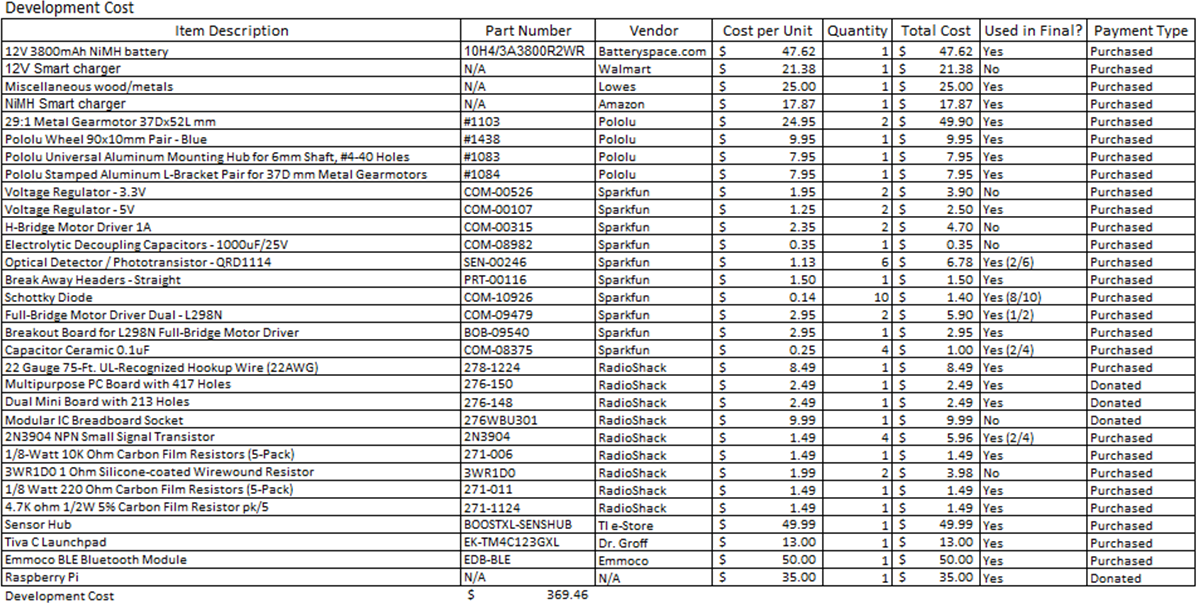
\includegraphics[width=\textwidth]{Costs1}
    \end{figure}
    \begin{figure}[H]
        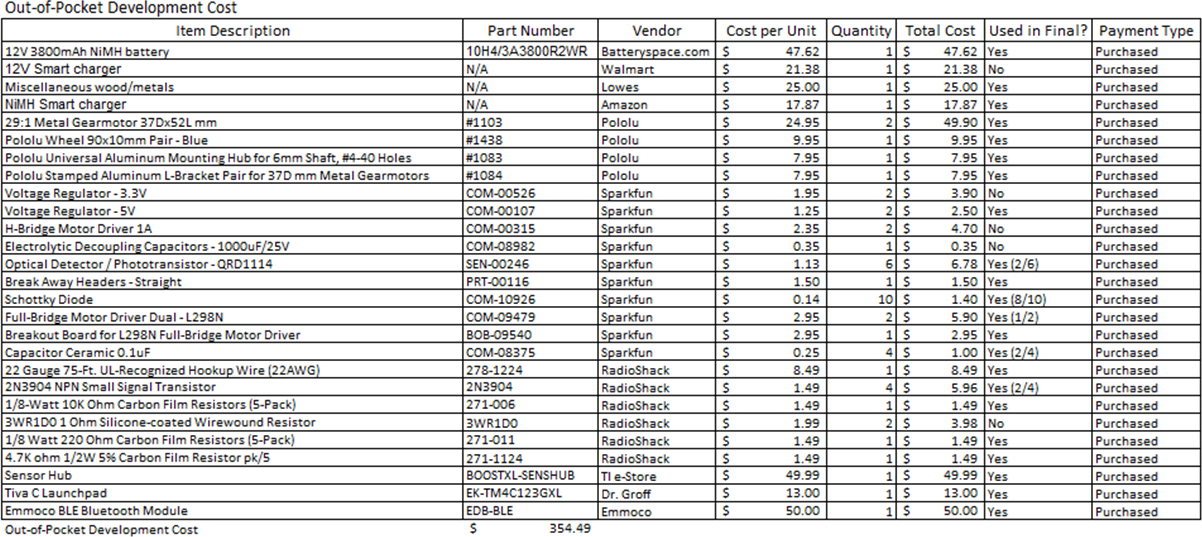
\includegraphics[width=\textwidth]{Costs2}
    \end{figure}
    \begin{figure}[H]
        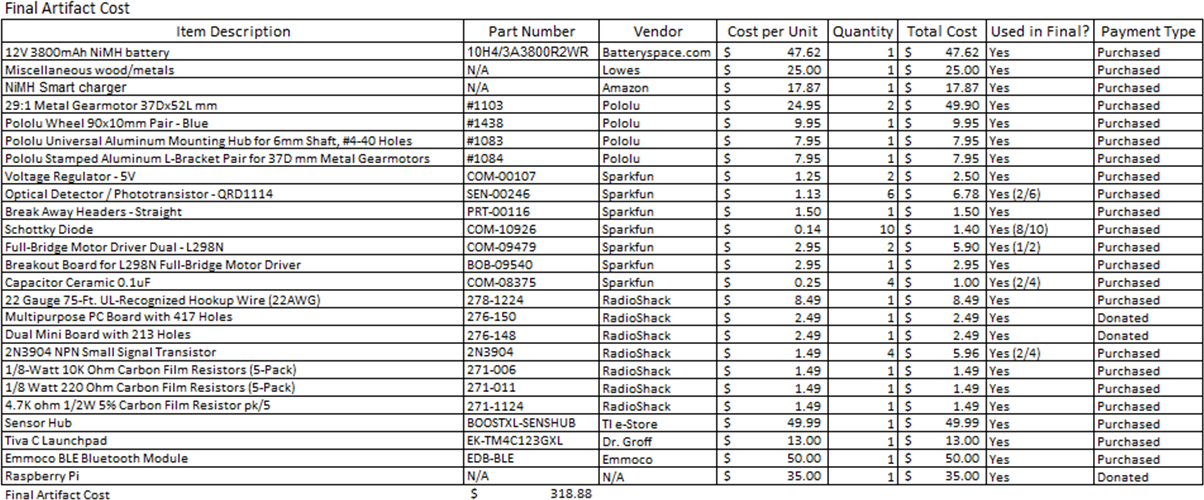
\includegraphics[width=\textwidth]{Costs3}
    \end{figure}
    \begin{figure}[H]
        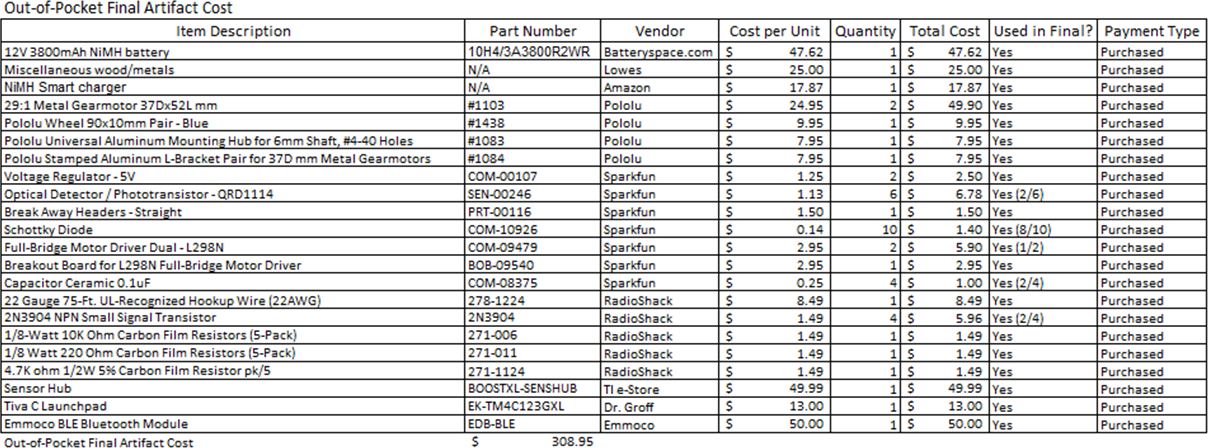
\includegraphics[width=\textwidth]{Costs4}
    \end{figure}

\clearpage

\section*{Appendix A: Root Locus Plots and Discussion}

Figure \ref{RootLocusOriginal} shows the root locus plot for the angular position to torque transfer function.  The pole in the right hand half of the plane never moves to the stable left hand side of the plane.  As such, a lead compensator was used to introduce a zero at -5 and a pole at 35 in order to force this pole into the left hand side of the plane.  The new root locus plot is shown in Figure \ref{RootLocusNew}.

\begin{figure}[H]
                \centering
                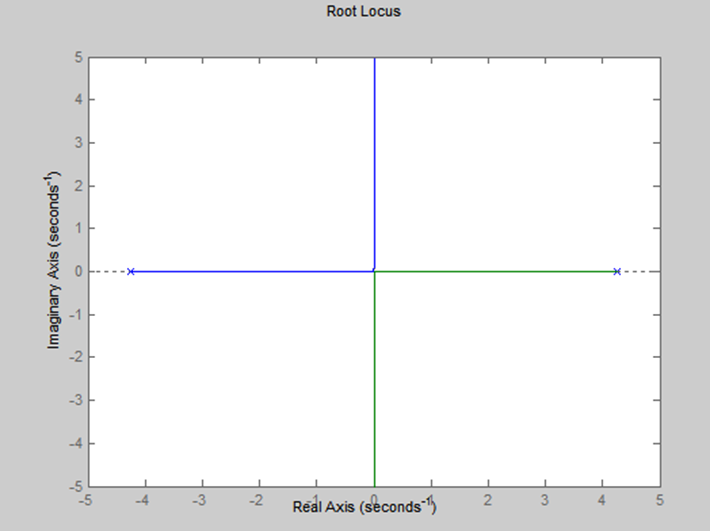
\includegraphics[width=0.5\textwidth]{RootLocusOriginal}
                \caption{Original Root Locus Plot}
                \label{RootLocusOriginal}
            \end{figure}

\begin{figure}[H]
                \centering
                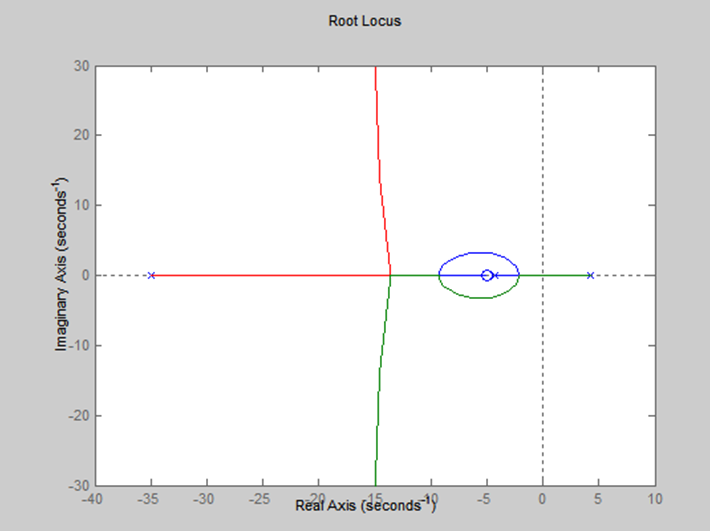
\includegraphics[width=0.5\textwidth]{RootLocusNew}
                \caption{New Root Locus Plot with Additional Zero and Pole}
                \label{RootLocusNew}
            \end{figure}

%% END EDITS HERE %%

\end{spacing}

\end{document}
